\documentclass[12pt]{article}
\usepackage[spanish]{babel}
\usepackage[utf8]{inputenc}
\usepackage{amsmath, amssymb}
\usepackage{graphicx}
\usepackage{fancyhdr}
\usepackage{titlesec}
\usepackage{geometry}
\geometry{a4paper, margin=2.5cm}
\usepackage{float}

\setlength{\headheight}{14.5pt}
\addtolength{\topmargin}{-2.5pt}

\titleformat{\section}{\large\bfseries}{\thesection.}{1em}{}
\pagestyle{fancy}
\fancyhf{}
\rhead{INF245 - Laboratorio 3}
\lhead{Don Bit y Bitópolis}
\rfoot{\thepage}

\title{\textbf{INF245 – Laboratorio 3} \\ Don Bit y Bitópolis}
\author{
    Sebastián Richiardi Pérez – 202030555-2 – 201\\
    Gabriel Alejandro Toro Varela – 202204557-4 – 201
}
\date{02 de junio de 2025}

\begin{document}

\maketitle

\newpage
\tableofcontents

\bigskip
\bigskip
\bigskip

\newpage

\section{Introducción}
En este laboratorio se implementa un sistema digital en Logisim para simular los recorridos dentro de la ciudad digital Bitópolis. Se emplea lógica secuencial sin memorias ROM/RAM, únicamente con compuertas lógicas y flip-flops tipo D, mostrando paso a paso el trayecto en un display de 7 segmentos.

\section{Descripción del problema}
Don Bit construyó una ciudad digital donde los vehículos se guían por un código de 4 bits que define un nodo inicial en un grafo. Cada uno de los 16 códigos posibles activa una ruta única y secuencial hacia el nodo final común: F.

\begin{figure}[H]
  \centering
  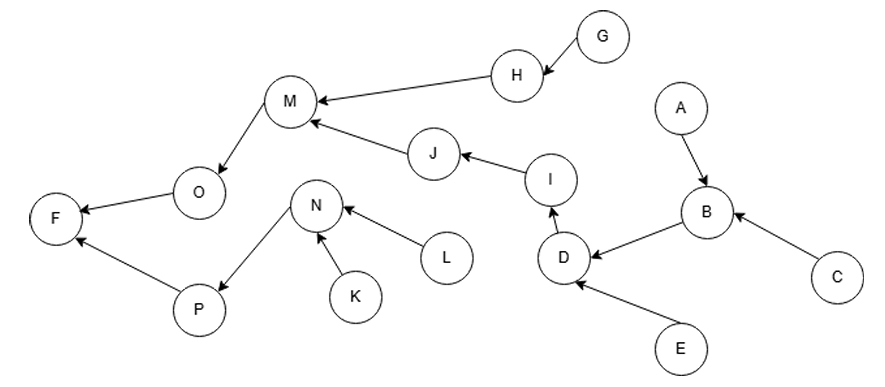
\includegraphics[width=0.7\textwidth]{.github/mapaderutas.png}
  \caption{Mapa de rutas del grafo de Bitópolis: cada nodo (A–P) tiene una única transición hacia el nodo final F.}
  \label{fig:mapaderutas}
\end{figure}

A partir del mapa de rutas presentado en la Figura \ref{fig:mapaderutas}, el objetivo es diseñar un circuito secuencial que, dado un nodo inicial en el rango \(\texttt{0000}_{2}\) a \(\texttt{1111}_{2}\) (correspondiente a las letras A–P), recorra automáticamente la única ruta predefinida hasta el nodo final \(F\). En cada estado intermedio del recorrido, el sistema debe mostrar el identificador del nodo actual en un display de 7 segmentos, usando un decodificador de 4 bits a 7 salidas (subcircuito \texttt{D7}).

\newpage
% -------------------------------------------------------
%    3. Diseño del sistema
% -------------------------------------------------------
\section{Diseño del sistema}

La máquina de estados finitos (FSM) se implementa en Logisim usando únicamente compuertas lógicas,
flip-flops tipo D y multiplexores, sin recurrir a memorias ROM/RAM. A continuación se describen
los bloques principales y cómo se relacionan:

\begin{enumerate}
  \item \textbf{StateRegister (Registro de estado)}:  
        Consta de cuatro flip-flops tipo D en paralelo que almacenan el “estado actual” 
        \(\,State[3..0]\). Este registro recibe en cada flanco de reloj el valor de entrada 
        proveniente de \texttt{MuxDeCarga}. Además cuenta con una señal de \texttt{Reset} asíncrona 
        que fuerza el valor “0000” (nodo \(\texttt{A}\)) cuando se activa, y con una entrada 
        \texttt{Enable} vinculada a \texttt{DetectF} para detener la captura una vez que se alcanza 
        el nodo final \(\texttt{F}\).  
        
  \item \textbf{MuxDeCarga (Multiplexor de carga)}:  
        Consta de cuatro multiplexores 2:1 (uno por cada bit) cuyo selector es la señal 
        \(\texttt{LOAD}\).  
        \begin{itemize}
          \item Si \(\texttt{LOAD}=1\), cada multiplexor deja pasar el bit correspondiente de
                \(\texttt{UserIn}[i]\) (entrada de 4 bits del usuario, nodo inicial).  
          \item Si \(\texttt{LOAD}=0\), deja pasar el bit correspondiente de 
                \(\texttt{NextState}[i]\).  
        \end{itemize}
        La salida de cada multiplexor (\(\texttt{D}[i]\)) se conecta a la entrada D de cada flip-flop
        en \texttt{StateRegister}.

  \item \textbf{NextState (Lógica combinacional 4 \(\to\) 4)}:  
        Toma como entrada los 4 bits \(\,State[3..0]\) (estado actual) y genera 4 bits 
        \(\,NextState[3..0]\), calculando el nodo sucesor según la ruta única predefinida.  
        En particular, cuando \(State = F\), se asegura que \(NextState = F\) para detener el avance.
        Esta lógica se puede implementar bien mediante mapas de Karnaugh y puertas lógicas, 
        o bien con cuatro multiplexores 16:1 que, seleccionados por \((State[3..0])\), indiquen 
        cada bit de \(\,NextState\).

  \item \textbf{DetectF (Detección de nodo final)}:  
        Bloque combinacional que compara \(\,State[3..0]\) con el valor binario correspondiente a 
        \(\texttt{F}\) (por ejemplo, \(\texttt{0101}_2\) si \(\texttt{F}=5\)).  
        Cuando coinciden, la salida \(\texttt{Finished}=1\). Esta señal alimenta el pin 
        \texttt{Enable} de \texttt{StateRegister} (o bien se utiliza para forzar 
        \(\,NextState(F)=F\)), de modo que, al llegar a \(\texttt{F}\), la FSM se “congela” 
        y no avanza más.

  \item \textbf{D7 (Decodificador 4 \(\to\) 7 segmentos)}:  
        Convierte los 4 bits \(\,State[3..0]\) en las 7 señales \((a,b,c,d,e,f,g)\) que activan 
        los segmentos del display para formar la letra del nodo actual (A–P).  
        De esta forma, en cada ciclo de reloj, el registro \(\texttt{State}\) actualiza la salida de 
        \texttt{D7}, y el display muestra la letra correspondiente.

  \item \textbf{Reloj (\texttt{CLK}) y control de carga (\texttt{LOAD})}:  
        \begin{itemize}
          \item La señal \texttt{CLK} es el pulso principal que sincroniza los flip-flops de 
                \texttt{StateRegister}.  
          \item La señal \(\texttt{LOAD}\) proviene de un botón o interruptor del usuario:  
            \begin{itemize}
              \item Cuando \(\texttt{LOAD}=1\), en el siguiente flanco ascendente de \(\texttt{CLK}\) 
                    se cargan los 4 bits de \(\texttt{UserIn}[3..0]\) en \(\texttt{StateRegister}\).  
              \item Inmediatamente después de ese pulso, el usuario deja \(\texttt{LOAD}=0\), y 
                    entonces \(\texttt{MuxDeCarga}\) conmuta a usar \(\texttt{NextState}\).  
            \end{itemize}
        \end{itemize}
\end{enumerate}

\subsection{Algoritmo general}

El comportamiento de la FSM se puede resumir en los siguientes pasos:

\begin{enumerate}
  \item \textbf{Entrada inicial:}  
        El usuario coloca, mediante interruptores, un valor binario de 4 bits 
        \(\,\texttt{UserIn}[3..0]\) (rango 0000–1111), que representa el nodo inicial \(S_{0}\).  
        
  \item \textbf{Carga del estado inicial:}  
        \begin{itemize}
          \item El usuario activa \(\texttt{LOAD} = 1\).  
          \item En el flanco ascendente de \(\texttt{CLK}\) siguiente, \(\texttt{MuxDeCarga}\) toma 
                \(\texttt{UserIn}\) y lo proporciona a las entradas \(\texttt{D}[3..0]\) de 
                \texttt{StateRegister}.  
          \item \texttt{StateRegister} almacena \(\,State \leftarrow \texttt{UserIn}\).  
        \end{itemize}

  \item \textbf{Inicio del recorrido:}  
        \(\texttt{LOAD}\) vuelve a 0 (botón suelto). Ahora, \(\texttt{MuxDeCarga}\) pasa a seleccionar 
        \(\texttt{NextState}[3..0]\) en lugar de \(\texttt{UserIn}\).  
        
  \item \textbf{Ciclo de transición:}  
        Repetir en cada flanco ascendente de \(\texttt{CLK}\) mientras \(\texttt{Finished} = 0\):  
        \begin{enumerate}
          \item \texttt{DetectF} comprueba si \(\,State = F\).  
            \begin{itemize}
              \item Si \(\,State \neq F\), \(\texttt{Finished} = 0\) y \(\texttt{Enable} = 1\).  
              \item Si \(\,State = F\), \(\texttt{Finished} = 1\) y \(\texttt{Enable} = 0\).  
            \end{itemize}
          \item Como \(\texttt{Enable} = 1\), en ese flanco de \(\texttt{CLK}\),  
            \(\texttt{StateRegister}\) actualiza  
            \[
              State \;\leftarrow\; NextState(State)\,,
            \]
            donde \(NextState(State)\) se obtiene de la lógica combinacional del bloque 
            \texttt{NextState}.  
          \item Automáticamente, los 4 bits de \(\,State\) pasan al bloque \texttt{D7},  
            el cual enciende los segmentos correspondientes para mostrar la letra  
            \(\{\texttt{A},\texttt{B},\dots,\texttt{P}\}\).  
        \end{enumerate}

  \item \textbf{Detención al llegar a \(F\):}  
        Cuando \(State = F\), el bloque \texttt{DetectF} pone \(\texttt{Finished} = 1\). Entonces  
        \(\texttt{Enable} = 0\) detiene la captura en \texttt{StateRegister} (o, alternativamente, 
        \(NextState(F)=F\) impide cualquier cambio). El valor \(F\) permanece en pantalla, 
        y el recorrido finaliza.

  \item \textbf{Visualización continua:}  
        Mientras \(\texttt{Finished} = 0\), cada nuevo valor de \(State\) (el nodo intermedio en la ruta)
        se muestra automáticamente en el display de 7 segmentos vía \texttt{D7}. Una vez que 
        \(\texttt{Finished} = 1\), la letra \(\texttt{F}\) permanece fija hasta que se active nuevamente  
        \texttt{Reset}.
\end{enumerate}

\begin{figure}[H]
  \centering
  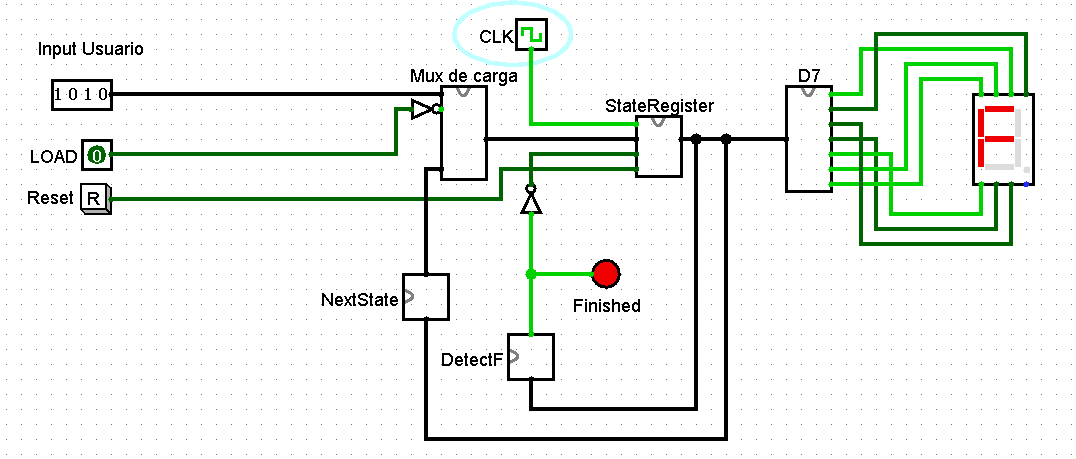
\includegraphics[width=0.8\textwidth]{.github/maincircuit.png}
  \caption{Diagrama general del sistema secuencial implementado en Logisim.}
  \label{fig:main_circuit}
\end{figure}

\noindent
\textbf{Descripción de los bloques en la Figura \ref{fig:main_circuit}:}
\begin{itemize}
  \item \textbf{StateRegister (4 D–FF)}: almacena el “estado actual” (\texttt{State[3..0]}).  
  \item \textbf{MuxDeCarga}: multiplexores 2:1 que eligen entre \(\texttt{UserIn}\) y 
        \(\texttt{NextState}\) según \(\texttt{LOAD}\).  
  \item \textbf{NextState (4 \(\to\) 4)}: lógica combinacional o MUXes 16:1 que calculan 
        \(\,NextState = f(State)\).  
  \item \textbf{DetectF (4 \(\to\) 1)}: comparador que genera \(\texttt{Finished}\) cuando 
        \(\,State = F\).  
  \item \textbf{D7 (4 \(\to\) 7)}: decodificador que convierte \(\,State\) en las señales 
        \((a,b,c,d,e,f,g)\) del display.  
  \item \(\texttt{CLK}\): señal de reloj que sincroniza \texttt{StateRegister} y \texttt{DetectF}.  
  \item \(\texttt{LOAD}\): botón que activa la carga inicial de \(\texttt{UserIn}\) en \texttt{StateRegister}.  
  \item \(\texttt{Reset}\): señal asíncrona que fuerza \(\,State \leftarrow 0000\) (nodo A).  
  \item \(\texttt{Finished}\): indicador (LED) que se enciende cuando se llega a \(F\).  
\end{itemize}


\newpage

\subsection{Subcircuito \texttt{Decodificador 7 segmentos}}


El subcircuito \texttt{D7} recibe como entrada el código en binario de 4\,bits  
\((s_{3},s_{2},s_{1},s_{0})\) que representa el nodo actual (A…P) y produce como salida  
el código en binario de 7\,bits \((a,b,c,d,f,g)\) correspondiente al segmento del display LED. 

% ---------------------------
% 3.4 Tabla de verdad del Decodificador 7 segmentos
% ---------------------------
\subsubsection{Tabla de verdad del subcircuito}

\begin{table}[ht]
\centering
\begin{tabular}{|c|c|c||c|c|c|c|c|c|c|}
\hline
\textbf{Dec} & \textbf{Binario} & \textbf{Nodo} 
  & \textbf{a} & \textbf{b} & \textbf{c} & \textbf{d} & \textbf{e} & \textbf{f} & \textbf{g} \\
\hline
0  & 0000 & A & 1 & 1 & 1 & 0 & 1 & 1 & 1 \\  
1  & 0001 & B & 0 & 0 & 1 & 1 & 1 & 1 & 1 \\  
2  & 0010 & C & 1 & 0 & 0 & 1 & 1 & 1 & 0 \\  
3  & 0011 & D & 0 & 1 & 1 & 1 & 1 & 0 & 1 \\  
4  & 0100 & E & 1 & 0 & 0 & 1 & 1 & 1 & 1 \\  
5  & 0101 & F & 1 & 0 & 0 & 0 & 1 & 1 & 1 \\  
6  & 0110 & G & 1 & 0 & 1 & 1 & 1 & 1 & 0 \\  
7  & 0111 & H & 0 & 1 & 1 & 0 & 1 & 1 & 1 \\  
8  & 1000 & I & 0 & 1 & 1 & 0 & 0 & 0 & 0 \\  
9  & 1001 & J & 0 & 1 & 1 & 1 & 1 & 0 & 0 \\  
10 & 1010 & K & 1 & 0 & 1 & 0 & 1 & 1 & 1 \\  
11 & 1011 & L & 0 & 0 & 0 & 1 & 1 & 1 & 0 \\  
12 & 1100 & M & 1 & 0 & 1 & 0 & 1 & 0 & 1 \\  
13 & 1101 & N & 1 & 0 & 1 & 0 & 1 & 0 & 0 \\  
14 & 1110 & O & 1 & 1 & 1 & 1 & 1 & 1 & 0 \\  
15 & 1111 & P & 1 & 1 & 0 & 0 & 1 & 1 & 1 \\  
\hline
\end{tabular}
\caption{Tabla de verdad del decodificador de 7 segmentos para nodos A–P.}
\label{tab:7seg_decoder}
\end{table}

% ---------------------------
% 3.4.1 Mapas de Karnaugh para el Decodificador 7 segmentos
% ---------------------------
\subsubsection{Mapas de Karnaugh para cada bit de salida}

\bigskip

\noindent
\textbf{Mapa K‐map de segmento \textsf{a}}  
\[
\begin{array}{c|cccc}
\multicolumn{1}{c}{x_3x_2 \backslash x_1x_0} & 00 & 01 & 11 & 10 \\
\hline
00 & 1 & 0 & 0 & 1 \\
01 & 1 & 1 & 0 & 1 \\
11 & 1 & 1 & 1 & 1 \\
10 & 0 & 0 & 0 & 1 \\
\end{array}
\]
\vspace{1em}

\noindent
\textbf{Función minimizada para \(a\):}
\[
x_3x_2 + x_2\overline{x_1} + \overline{x_3}\,\overline{x_1}\,\overline{x_0} + x_1\,\overline{x_0}
\]

\noindent
\textbf{Mapa K‐map de segmento \textsf{b}}  
\[
\begin{array}{c|cccc}
\multicolumn{1}{c}{x_3x_2 \backslash x_1x_0} & 00 & 01 & 11 & 10 \\
\hline
00 & 1 & 0 & 1 & 0 \\
01 & 0 & 0 & 1 & 0 \\
11 & 1 & 0 & 1 & 1 \\
10 & 1 & 1 & 0 & 0 \\
\end{array}
\]
\vspace{1em}

\noindent
\textbf{Función minimizada para \(b\):}
\[
\overline{x_2}\,\overline{x_1}\,\overline{x_0} + x_3\,\overline{x_2}\,\overline{x_1} + \overline{x_3}\,x_1\,x_0 + x_2\,x_1\,x_0 + x_3\,x_2\,x_1
\]

\noindent
\textbf{Mapa K‐map de segmento \textsf{c}}  
\[
\begin{array}{c|cccc}
\multicolumn{1}{c}{x_3x_2 \backslash x_1x_0} & 00 & 01 & 11 & 10 \\
\hline
00 & 1 & 1 & 1 & 0 \\
01 & 0 & 0 & 1 & 1 \\
11 & 1 & 1 & 0 & 1 \\
10 & 1 & 1 & 0 & 1 \\
\end{array}
\]
\vspace{1em}

\noindent
\textbf{Función minimizada para \(c\):}
\[
\overline{x_2}\,\overline{x_1} + \overline{x_3}\,\overline{x_2}\,x_0 + \overline{x_3}\,x_2\,x_1 + x_3\,x_1\,\overline{x_0} + x_3\,x_2\,\overline{x_1}
\]

\noindent
\textbf{Mapa K‐map de segmento \textsf{d}}  
\[
\begin{array}{c|cccc}
\multicolumn{1}{c}{x_3x_2 \backslash x_1x_0} & 00 & 01 & 11 & 10 \\
\hline
00 & 0 & 1 & 1 & 1 \\
01 & 1 & 0 & 0 & 1 \\
11 & 0 & 0 & 0 & 1 \\
10 & 0 & 1 & 1 & 0 \\
\end{array}
\]
\vspace{1em}

\noindent
\textbf{Función minimizada para \(d\):}
\[
\overline{x_3}\,x_1\,\overline{x_0} + \overline{x_3}\,\overline{x_2}\,x_1 + x_2\,x_1\,\overline{x_0} + \overline{x_3}\,\overline{x_2}\,x_0 + x_3\,\overline{x_2}\,x_0 + \overline{x_3}\,x_2\,\overline{x_1}\,\overline{x_0}
\]

\noindent
\textbf{Mapa K‐map de segmento \textsf{e}}  
\[
\begin{array}{c|cccc}
\multicolumn{1}{c}{x_3x_2 \backslash x_1x_0} & 00 & 01 & 11 & 10 \\
\hline
00 & 1 & 1 & 1 & 1 \\
01 & 1 & 1 & 1 & 1 \\
11 & 1 & 1 & 1 & 1 \\
10 & 0 & 1 & 1 & 1 \\
\end{array}
\]
\vspace{1em}

\noindent
\textbf{Función minimizada para \(e\):}
\[
\overline{x_3} + x_2 + x_1 + x_0
\]

\noindent
\textbf{Mapa K‐map de segmento \textsf{f}}  
\[
\begin{array}{c|cccc}
\multicolumn{1}{c}{x_3x_2 \backslash x_1x_0} & 00 & 01 & 11 & 10 \\
\hline
00 & 1 & 1 & 0 & 1 \\
01 & 1 & 1 & 1 & 1 \\
11 & 0 & 0 & 1 & 1 \\
10 & 0 & 0 & 1 & 1 \\
\end{array}
\]
\vspace{1em}

\noindent
\textbf{Función minimizada para \(f\):}
\[
x_3\,x_1 + \overline{x_3}\,x_2 + \overline{x_3}\,\overline{x_2}\,\overline{x_1} + x_1\,\overline{x_0}
\]

\noindent
\textbf{Mapa K‐map de segmento \textsf{g}}  
\[
\begin{array}{c|cccc}
\multicolumn{1}{c}{x_3x_2 \backslash x_1x_0} & 00 & 01 & 11 & 10 \\
\hline
00 & 1 & 1 & 1 & 0 \\
01 & 1 & 1 & 1 & 0 \\
11 & 1 & 0 & 1 & 0 \\
10 & 0 & 0 & 0 & 1 \\
\end{array}
\]
\vspace{1em}

\noindent
\textbf{Función minimizada para \(g\):}
\[
\overline{x_3}\,\overline{x_1} + \overline{x_3}\,x_1\,x_0 + x_2\,\overline{x_1}\,\overline{x_0} + x_2\,x_1\,x_0 + x_3\,\overline{x_2}\,x_1\,\overline{x_0}
\]

\newpage

% ------------------------------------------------------------
% Subcircuito “NextState”: tabla de verdad, mapas de Karnaugh y funciones minimizadas
% ------------------------------------------------------------

\subsection{Subcircuito \texttt{NextState}}

El subcircuito \texttt{NextState} recibe como entrada el código en binario de 4\,bits  
\((s_{3},s_{2},s_{1},s_{0})\) que representa el nodo actual (A…P) y produce como salida  
el código en binario de 4\,bits \((n_{3},n_{2},n_{1},n_{0})\) correspondiente al siguiente nodo en la ruta. 

\subsubsection{Tabla de verdad del subcircuito}
% ------------------------------------------------------------
% 1) Tabla de verdad del subcircuito NextState
% ------------------------------------------------------------
\begin{table}[H]
  \centering
  \begin{tabular}{cccc|cccc}
    \multicolumn{4}{c|}{\bf Estado presente} & \multicolumn{4}{c}{\bf NextState}\\
    \multicolumn{4}{c|}{\((s_{3}\;\;s_{2}\;\;s_{1}\;\;s_{0})\)} & \multicolumn{4}{c}{\((n_{3}\;\;n_{2}\;\;n_{1}\;\;n_{0})\)}\\
    \hline
    0 & 0 & 0 & 0 & 0 & 0 & 0 & 1 \\ % A → B
    0 & 0 & 0 & 1 & 0 & 0 & 1 & 1 \\ % B → D
    0 & 0 & 1 & 0 & 0 & 0 & 0 & 1 \\ % C → B
    0 & 0 & 1 & 1 & 1 & 0 & 0 & 0 \\ % D → I
    0 & 1 & 0 & 0 & 0 & 0 & 1 & 1 \\ % E → D
    0 & 1 & 0 & 1 & 0 & 1 & 0 & 1 \\ % F → F
    0 & 1 & 1 & 0 & 0 & 1 & 1 & 1 \\ % G → H
    0 & 1 & 1 & 1 & 1 & 1 & 0 & 0 \\ % H → M
    1 & 0 & 0 & 0 & 1 & 0 & 0 & 1 \\ % I → J
    1 & 0 & 0 & 1 & 1 & 1 & 0 & 0 \\ % J → M
    1 & 0 & 1 & 0 & 1 & 1 & 0 & 1 \\ % K → N
    1 & 0 & 1 & 1 & 1 & 1 & 0 & 1 \\ % L → N
    1 & 1 & 0 & 0 & 1 & 1 & 1 & 0 \\ % M → O
    1 & 1 & 0 & 1 & 1 & 1 & 1 & 1 \\ % N → P
    1 & 1 & 1 & 0 & 0 & 1 & 0 & 1 \\ % O → F
    1 & 1 & 1 & 1 & 0 & 1 & 0 & 1 \\ % P → F
  \end{tabular}
  \caption{Tabla de verdad del subcircuito \texttt{NextState}. Cada fila indica la transición  
    desde el estado presente \((s_{3}\,s_{2}\,s_{1}\,s_{0})\) al siguiente \((n_{3}\,n_{2}\,n_{1}\,n_{0})\).}
\end{table}

\bigskip

% ------------------------------------------------------------
% 2) Mapas de Karnaugh
% ------------------------------------------------------------

\subsubsection{Mapas de Karnaugh para cada bit de salida}

Se usarán mapas de Karnaugh 4×4 con la convención Gray en filas \((s_3\,s_2)\) y columnas \((s_1\,s_0)\).  

\paragraph*{(a) Mapa de Karnaugh para \(n_{3}(s_{3},s_{2},s_{1},s_{0})\).}

\begin{center}
\begin{tabular}{c|cccc}
  \multicolumn{1}{c}{} & \multicolumn{4}{c}{\((s_{1}\,s_{0})\)} \\[-2pt]
  \cline{2-5}
  \((s_{3}\,s_{2})\) & 00 & 01 & 11 & 10 \\
  \cline{1-5}
  00 & 0 & 0 & \bf1 & 0 \\  % minterm 3
  01 & 0 & 0 & \bf1 & 0 \\  % minterm 7
  11 & \bf1 & \bf1 & 0 & 0 \\% minterms 12, 13
  10 & \bf1 & \bf1 & \bf1 & \bf1 \\ % minterms 8,9,11,10
  \cline{1-5}
\end{tabular}
\end{center}

\noindent
\textbf{Agrupaciones:}
\begin{itemize}
  \item \(\{8,9,11,10\}\) (fila \(s_{3}s_{2}=10\) entera) \(\;\longrightarrow\; s_{3}\,\overline{s_{2}}\).
  \item \(\{8,9,12,13\}\) (\(\,(s_{3}s_{2})\in\{10,11\},\,(s_{1}s_{0})\in\{00,01\}\))  
    \(\;\longrightarrow\; s_{3}\,\overline{s_{1}}\).
  \item \(\{3,7\}\) (\((s_{3}s_{2})\in\{00,01\},\,(s_{1}s_{0})=11\))  
    \(\;\longrightarrow\; \overline{s_{3}}\,s_{1}\,s_{0}\).
\end{itemize}

\noindent
\textbf{Función minimizada para \(n_{3}\):}
\[
  n_{3} \;=\; 
    \underbrace{s_{3}\,\overline{s_{2}}}_{\text{(fila 10)}} 
    \;+\; 
    \underbrace{s_{3}\,\overline{s_{1}}}_{\substack{\text{(filas 10–11 en}\\(s_{1}s_{0})\in\{00,01\})}} 
    \;+\; 
    \underbrace{\overline{s_{3}}\,s_{1}\,s_{0}}_{\text{(columnas 11)}}.
\]

\bigskip

\paragraph*{(b) Mapa de Karnaugh para \(n_{2}(s_{3},s_{2},s_{1},s_{0})\).}

\begin{center}
\begin{tabular}{c|cccc}
  \multicolumn{1}{c}{} & \multicolumn{4}{c}{\((s_{1}\,s_{0})\)} \\[-2pt]
  \cline{2-5}
  \((s_{3}\,s_{2})\) & 00 & 01 & 11 & 10 \\
  \cline{1-5}
  00 & 0 & 0 & 0 & 0 \\ 
  01 & 0 & \bf1 & \bf1 & \bf1 \\ % minterms 5,7,6
  11 & \bf1 & \bf1 & \bf1 & \bf1 \\% minterms 12,13,15,14
  10 & 0 & \bf1 & \bf1 & \bf1 \\ % minterms 9,11,10
  \cline{1-5}
\end{tabular}
\end{center}

\noindent
\textbf{Agrupaciones:}
\begin{itemize}
  \item \(\{12,13,15,14\}\) (fila \(s_{3}s_{2}=11\) entera)  
    \(\;\longrightarrow\; s_{3}\,s_{2}.\)
  \item \(\{6,7,15,14\}\) (\((s_{3}s_{2})\in\{01,11\},\,(s_{1}s_{0})\in\{11,10\}\))  
    \(\;\longrightarrow\; s_{2}\,s_{1}.\)
  \item \(\{6,7,11,10\}\) (\((s_{3}s_{2})\in\{01,10\},\,(s_{1}s_{0})\in\{11,10\}\))  
    \(\;\longrightarrow\; s_{1}.\)
  \item \(\{9,13\}\) (\((s_{3}s_{2})\in\{10,11\},\,(s_{1}s_{0})=01\))  
    \(\;\longrightarrow\; s_{3}\,s_{0}.\)
  \item \(\{10,14\}\) (\((s_{3}s_{2})\in\{10,11\},\,(s_{1}s_{0})=10\))  
    \(\;\longrightarrow\; s_{2}\,s_{0}.\)
\end{itemize}

\noindent
\textbf{Función minimizada para \(n_{2}\):}
\[
  n_{2} \;=\; 
    \underbrace{s_{3}\,s_{2}}_{\{12,13,15,14\}} 
    \;+\; 
    \underbrace{s_{2}\,s_{1}}_{\{6,7,15,14\}} 
    \;+\; 
    \underbrace{s_{1}}_{\{6,7,11,10\}} 
    \;+\; 
    \underbrace{s_{3}\,s_{0}}_{\{9,13\}} 
    \;+\; 
    \underbrace{s_{2}\,s_{0}}_{\{10,14\}}.
\]

\bigskip

\paragraph*{(c) Mapa de Karnaugh para \(n_{1}(s_{3},s_{2},s_{1},s_{0})\).}

\begin{center}
\begin{tabular}{c|cccc}
  \multicolumn{1}{c}{} & \multicolumn{4}{c}{\((s_{1}\,s_{0})\)} \\[-2pt]
  \cline{2-5}
  \((s_{3}\,s_{2})\) & 00 & 01 & 11 & 10 \\
  \cline{1-5}
  00 & 0 & \bf1 & 0 & 0 \\   % minterm 1
  01 & \bf1 & 0 & 0 & \bf1 \\% minterms 4,6
  11 & \bf1 & \bf1 & 0 & 0 \\% minterms 12,13
  10 & 0 & 0 & 0 & 0 \\ 
  \cline{1-5}
\end{tabular}
\end{center}

\noindent
\textbf{Agrupaciones:}
\begin{itemize}
  \item \(\{4,12\}\) (fila \(s_{3}s_{2}=01,11\), columna “00”):  
    \[
      s_{1}=0,\;s_{0}=0,\;s_{2}=1,\;(s_{3}\text{ varía})  
      \;\longrightarrow\; s_{2}\,\overline{s_{1}}\,\overline{s_{0}}.
    \]
  \item \(\{12,13\}\) (fila \(s_{3}s_{2}=11\), columnas \(\{00,01\}\)):  
    \[
      s_{3}=1,\;s_{2}=1,\;s_{1}=0,\;(s_{0}\text{ varía})  
      \;\longrightarrow\; s_{3}\,s_{2}\,\overline{s_{1}}.
    \]
  \item \(\{6\}\) (aislado en fila “01”, columna “10”):  
    \[
      (s_{3},s_{2},s_{1},s_{0}) = (0,1,1,0)  
      \;\longrightarrow\; \overline{s_{3}}\,s_{2}\,s_{1}\,\overline{s_{0}}.
    \]
  \item \(\{1\}\) (aislado en fila “00”, columna “01”):  
    \[
      (s_{3},s_{2},s_{1},s_{0}) = (0,0,0,1)  
      \;\longrightarrow\; \overline{s_{3}}\,\overline{s_{2}}\,\overline{s_{1}}\,s_{0}.
    \]
\end{itemize}

\noindent
\textbf{Función minimizada para \(n_{1}\):}
\[
  n_{1} 
  \;=\; 
    \underbrace{\bigl(\overline{s_{3}}\,s_{2}\,\overline{s_{0}}\bigr)}_{\{4,6\}} 
    \;+\; 
    \underbrace{\bigl(s_{3}\,s_{2}\,\overline{s_{1}}\bigr)}_{\{12,13\}} 
    \;+\; 
    \underbrace{\bigl(\overline{s_{3}}\,\overline{s_{2}}\,\overline{s_{1}}\,s_{0}\bigr)}_{\{1\}}.
\]

\bigskip

\paragraph*{(d) Mapa de Karnaugh para \(n_{0}(s_{3},s_{2},s_{1},s_{0})\).}

\begin{center}
\begin{tabular}{c|cccc}
  \multicolumn{1}{c}{} & \multicolumn{4}{c}{\((s_{1}\,s_{0})\)} \\[-2pt]
  \cline{2-5}
  \((s_{3}\,s_{2})\) & 00 & 01 & 11 & 10 \\
  \cline{1-5}
  00 & \bf1 & \bf1 & 0 & \bf1 \\   % minterms 0,1,2
  01 & \bf1 & \bf1 & 0 & \bf1 \\   % minterms 4,5,6
  11 & 0    & \bf1 & \bf1 & \bf1 \\% minterms 13,14,15
  10 & \bf1 & 0    & \bf1 & \bf1 \\% minterms 8,10,11
  \cline{1-5}
\end{tabular}
\end{center}

\noindent
\textbf{Agrupaciones:}
\begin{itemize}
  \item \(\{0,1,4,5\}\) (filas “00–01”, columnas “00–01”):  
    \(\;s_{3}=0,\;s_{1}=0\;\longrightarrow\;\overline{s_{3}}\,\overline{s_{1}}\).
  \item \(\{0,2,4,6\}\) (imbuída: filas “00–01”, columnas “00–10” (envolvente)):  
    \(\;s_{3}=0,\;s_{0}=0\;\longrightarrow\;\overline{s_{3}}\,\overline{s_{0}}\).
  \item \(\{10,11,14,15\}\) (filas “10–11”, columnas “10–11”):  
    \(\;s_{3}=1,\;s_{1}=1\;\longrightarrow\;s_{3}\,s_{1}\).
  \item \(\{8,10\}\) (fila “10”, columnas “00–10”):  
    \(\;s_{3}=1,\;s_{0}=0\;\longrightarrow\;s_{3}\,\overline{s_{0}}\).
  \item \(\{13\}\) (aislado en fila “11”, columna “01”):  
    \(\;(s_{3},s_{2},s_{1},s_{0})=(1,1,0,1)\;\longrightarrow\;s_{3}\,s_{2}\,\overline{s_{1}}\,s_{0}.\)
\end{itemize}

\noindent
\textbf{Función minimizada para \(n_{0}\):}
\[
  n_{0} 
  \;=\; 
    \underbrace{\bigl(\overline{s_{3}}\,\overline{s_{1}}\bigr)}_{p_{1}} 
    \;+\; 
    \underbrace{\bigl(\overline{s_{3}}\,\overline{s_{0}}\bigr)}_{p_{2}} 
    \;+\; 
    \underbrace{\bigl(s_{3}\,s_{1}\bigr)}_{p_{3}} 
    \;+\; 
    \underbrace{\bigl(s_{3}\,\overline{s_{0}}\bigr)}_{p_{5}} 
    \;+\; 
    \underbrace{\bigl(s_{3}\,s_{2}\,\overline{s_{1}}\,s_{0}\bigr)}_{p_{6}}.
\]

\bigskip

% ------------------------------------------------------------
% 3) Resumen de las funciones lógicas
% ------------------------------------------------------------

\subsubsection{Funciones lógicas minimizadas finales}

Finalmente, las cuatro salidas \((n_{3},n_{2},n_{1},n_{0})\) se describen mediante:

\[
\begin{aligned}
  n_{3}(s_{3},s_{2},s_{1},s_{0})
  &=\, s_{3}\,\overline{s_{2}}
    \;+\; s_{3}\,\overline{s_{1}}
    \;+\; \overline{s_{3}}\,s_{1}\,s_{0},\\[6pt]
  n_{2}(s_{3},s_{2},s_{1},s_{0})
  &=\, s_{3}\,s_{2}
    \;+\; s_{2}\,s_{1}
    \;+\; s_{1}
    \;+\; s_{3}\,s_{0}
    \;+\; s_{2}\,s_{0},\\[6pt]
  n_{1}(s_{3},s_{2},s_{1},s_{0})
  &=\, \overline{s_{3}}\,s_{2}\,\overline{s_{0}}
    \;+\; s_{3}\,s_{2}\,\overline{s_{1}}
    \;+\; \overline{s_{3}}\,\overline{s_{2}}\,\overline{s_{1}}\,s_{0},\\[6pt]
  n_{0}(s_{3},s_{2},s_{1},s_{0})
  &=\, \overline{s_{3}}\,\overline{s_{1}}
    \;+\; \overline{s_{3}}\,\overline{s_{0}}
    \;+\; s_{3}\,s_{1}
    \;+\; s_{3}\,\overline{s_{0}}
    \;+\; s_{3}\,s_{2}\,\overline{s_{1}}\,s_{0}.
\end{aligned}
\]

\newpage

% ---------------------------
% Subcircuito: MuxDeCarga
% ---------------------------
\subsection{Subcircuito \texttt{MuxDeCarga}}

El subcircuito \texttt{MuxDeCarga} es responsable de seleccionar, en cada ciclo de reloj, 
si el registro principal debe cargar la entrada del usuario (nodo inicial) o bien el valor 
proporcionado por la lógica \texttt{NextState}. Para lograr esto, se implementa un multiplexor 
de 2 a 1 para cada uno de los cuatro bits. Cuando la señal \texttt{LOAD} está activa, se elige 
la entrada del usuario; en caso contrario, se deja pasar la salida de \texttt{NextState}. 
La figura \ref{fig:muxdecarga} muestra el diagrama de este bloque.

\begin{figure}[H]
  \centering
  % Sustituye ".github/muxdecarga.png" por el nombre real del archivo de imagen que hayas generado
  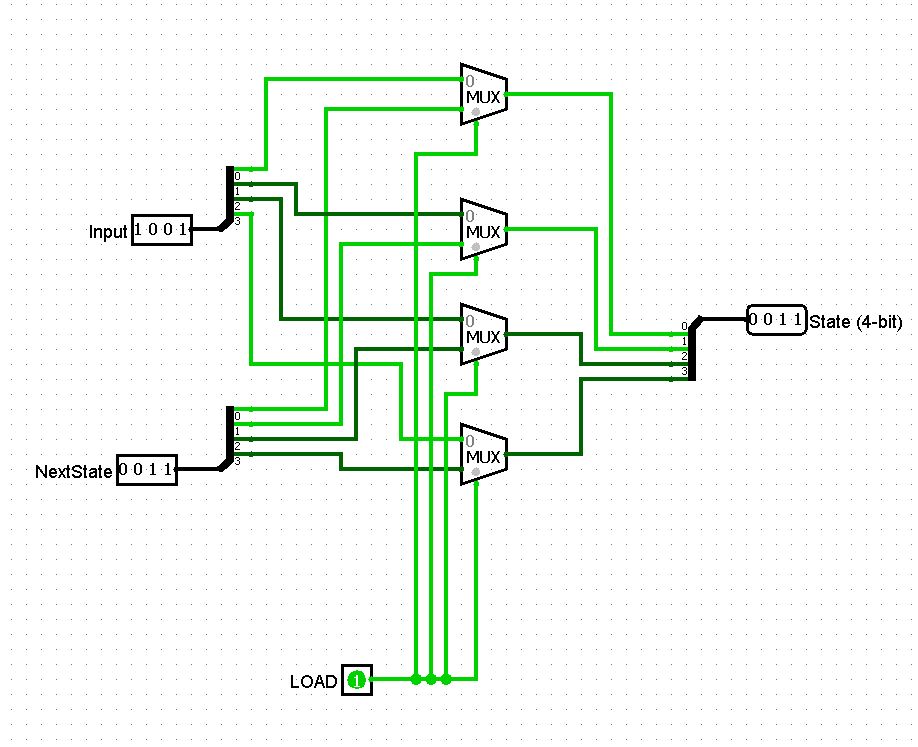
\includegraphics[width=0.6\textwidth]{.github/muxdecarga.png}
  \caption{Subcircuito \texttt{MuxDeCarga}: selección entre entrada de usuario y NextState.}
  \label{fig:muxdecarga}
\end{figure}

En pseudocódigo o en forma de tabla de verdad, su funcionamiento es:
\begin{itemize}
  \item \textbf{Entradas:} 
    \begin{itemize}
      \item \texttt{LOAD} (bit de control).
      \item \texttt{UserIn[3..0]} (interruptores del usuario, nodo inicial).
      \item \texttt{NextState[3..0]} (salida combinacional que indica el siguiente estado).
    \end{itemize}
  \item \textbf{Salidas:} 
    \begin{itemize}
      \item \texttt{D[3..0]} (bits que alimentan el registro de estado).
    \end{itemize}
  \item \textbf{Tabla de selección (por bit):}
    \[
      D[i] \;=\;
      \begin{cases}
        \texttt{UserIn}[i], & \text{si } \texttt{LOAD} = 1,\\
        \texttt{NextState}[i], & \text{si } \texttt{LOAD} = 0.
      \end{cases}
      \quad (i = 0,1,2,3)
    \]
\end{itemize}

Internamente, se usan cuatro puertas MUX 2:1 (una por cada bit) tal como se ilustra en la figura.

\newpage

% ---------------------------
% Subcircuito: DetectF
% ---------------------------
\subsection{Subcircuito \texttt{DetectF}}

El subcircuito \texttt{DetectF} detecta cuándo el registro de estado ha alcanzado el nodo
final \(F\). En nuestro diseño, consideramos que \(F\) está codificado en 4 bits —por ejemplo,
\(F = 0101_{2}\) si el nodo final es \(\text{F} = 5\). Cuando el estado actual coincide con
ese valor, la salida de \texttt{DetectF} se pone a 1 (“\texttt{Finished} = 1”), lo cual se usa
para, opcionalmente, detener el avance del registro (pasando \(\texttt{Enable} = 0\) a los flip-flops).
La figura \ref{fig:detectf} muestra el diagrama de este comparador.

\begin{figure}[H]
  \centering
  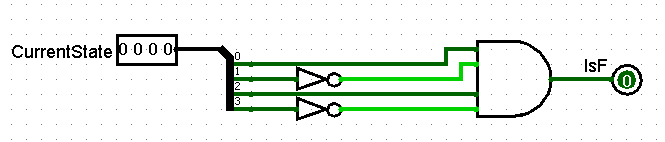
\includegraphics[width=0.45\textwidth]{.github/detectf.png}
  \caption{Subcircuito \texttt{DetectF}: compara el estado con el valor de \(\text{F}\).}
  \label{fig:detectf}
\end{figure}

\noindent
\textbf{Descripción del funcionamiento:}
\begin{itemize}
  \item \textbf{Entradas:} \(\,State[3..0]\) (codificación binaria del nodo actual).
  \item \textbf{Salida:} \(\texttt{Finished} = 1\) si y solo si \(State = F\). 
  \item \textbf{Implementación típica:}  
    \[
      \texttt{Finished} 
      \;=\;\bigl( \overline{State_{3}} \bigl) \;\wedge\; State_{2} \;\wedge\; \overline{State_{1}} \;\wedge\; State_{0}
      \quad
      (\text{si } F = 0101_{2}),
    \]
    donde cada literal (p. ej. \(\overline{State_{3}}\)) se obtiene con un inversor.
\end{itemize}

Adicionalmente, la señal \(\texttt{Finished}\) se conecta al pin de \texttt{Enable} de los
flip-flops de \texttt{StateRegister} para “congelar” el estado final y evitar más transiciones.


\newpage

% ---------------------------
% Subcircuito: StateRegister
% ---------------------------
\subsection{Subcircuito \texttt{StateRegister}}

El subcircuito \texttt{StateRegister} consta de cuatro flip-flops tipo D sincronizados con el
reloj \(\texttt{CLK}\). Cada flip-flop almacena uno de los bits del “estado actual” 
\(\,State[3..0]\). El registro recibe su entrada (\(\texttt{D}[3..0]\)) directamente desde 
\texttt{MuxDeCarga}. La señal de \(\texttt{Reset}\) asíncrona se utiliza para inicializar el registro en 
“0000” (nodo A) en el momento deseado, y la señal \(\texttt{Enable}\) (opcional) se activa con 
\(\overline{\texttt{Finished}}\) para detener el registro al llegar a \(F\). En la figura \ref{fig:stateregister} 
se muestra su circuito en logisim.

\begin{figure}[H]
  \centering
  % Sustituye ".github/stateregister.png" por el nombre real del archivo de imagen que hayas generado
  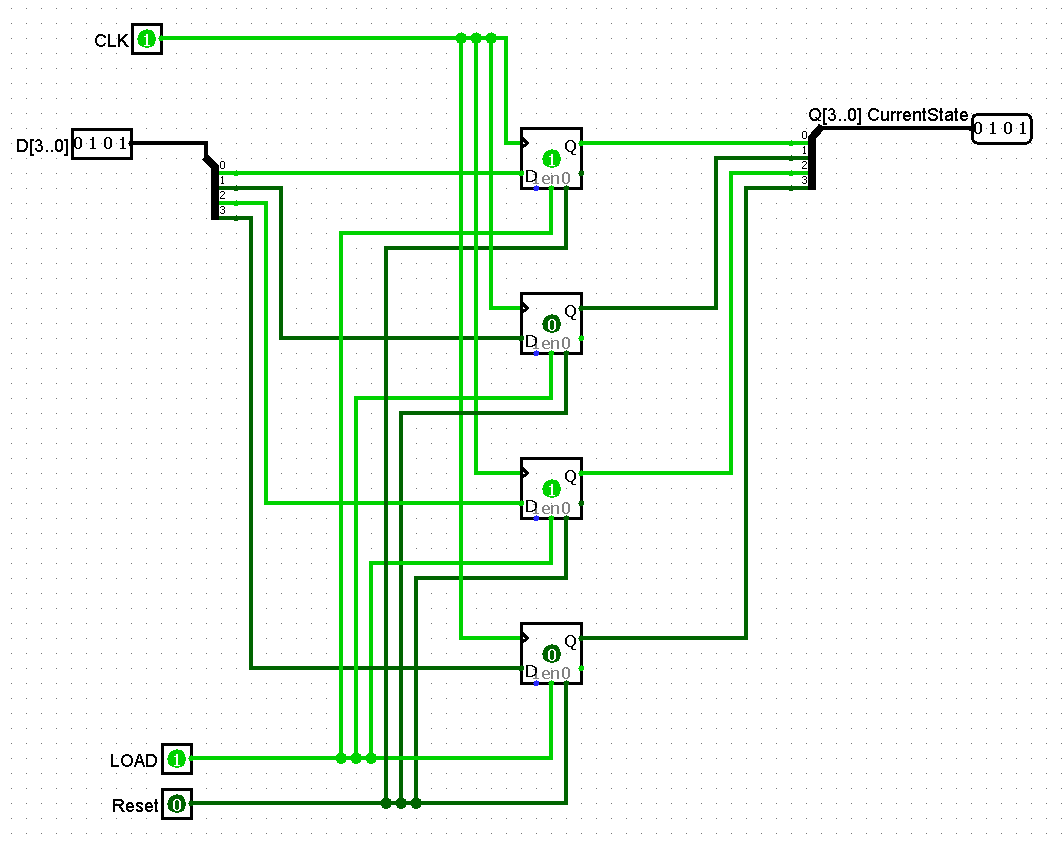
\includegraphics[width=0.55\textwidth]{.github/stateregister.png}
  \caption{Subcircuito \texttt{StateRegister}: cuatro D-Flip-Flops con Reset y Enable.}
  \label{fig:stateregister}
\end{figure}

\noindent
\textbf{Pines de control:}
\begin{itemize}
  \item \textbf{CLK:} Reloj principal (flanco ascendente) que sincroniza cada flip-flop.  
  \item \textbf{Reset:} Señal asíncrona para forzar \(\,State \leftarrow 0000\).  
  \item \textbf{Enable:} (opcional) \(\,=\overline{\texttt{Finished}}\). Cuando \(\texttt{Finished}=1\), 
    el registro deja de capturar flancos de reloj y mantiene el estado final \(F\).  
  \item \textbf{D[3..0]:} Bits de entrada, provenientes de \texttt{MuxDeCarga}.  
  \item \textbf{Q[3..0]:} Salida actual (\texttt{State}), que retroalimenta a \texttt{NextState} y \texttt{DetectF}, 
    y también se envía a \texttt{D7} para el display de 7 segmentos.
\end{itemize}

Cada flip-flop almacena un bit \(State_i\).
\newpage

\section{Supuestos}
\begin{itemize}
    \item No se requiere retroceso ni manejo de errores en tiempo real.
    \item El sistema parte desde reposo y no repite el ciclo una vez finalizado.
\end{itemize}

% ─────────────────────────────────────────────────────────────────────────────
%  Sección: Conclusión
% ─────────────────────────────────────────────────────────────────────────────
\section{Conclusión}

En este informe se ha presentado el diseño completo de un circuito secuencial capaz de recibir un código de 4 bits (valor de 0 a 15) que identifica un nodo de inicio en la ciudad digital de Bitópolis, recorrer automáticamente la ruta única y predefinida hacia el nodo final \texttt{F}, y mostrar en un display de 7 segmentos cada nodo visitado en cada pulso de reloj. 

Para ello, se desglosó la solución en los siguientes bloques:
\begin{enumerate}
    \item \textbf{MuxDeCarga}, que permite seleccionar entre el valor ingresado por el usuario o el valor calculado por \textit{NextState}.  
    \item \textbf{StateRegister}, formado por cuatro flip-flops tipo D, que almacenan el estado actual (nodo en curso) y avanzan de acuerdo al reloj.  
    \item \textbf{DetectF}, que detecta cuándo el estado coincide con el nodo final \texttt{F} para encender el indicador \texttt{Finished} y detener el recorrido.  
    \item \textbf{NextState}, la lógica combinacional que, dado el estado actual, calcula el siguiente nodo.  
    \item \textbf{Decodificador D7}, que traduce el código de 4 bits en las siete líneas necesarias para encender el display y mostrar la letra correspondiente al nodo actual.  
\end{enumerate}

El uso de flip-flops tipo D, multiplexores y puertas lógicas cumple con la restricción de no emplear memorias ROM/RAM ni otros tipos de flip-flops. Además, la señal \texttt{LOAD} (activada o negada según la implementación elegida) permite tanto la carga inicial del nodo como el pase a la ejecución automática de la secuencia. El LED \texttt{Finished} indica la finalización del recorrido sin entrar en bucle, y el botón \texttt{Reset} ofrece un mecanismo sencillo para reiniciar el sistema a \texttt{0000} en cualquier momento.

Finalmente, la modularización en los subcircuitos \texttt{MuxDeCarga}, \texttt{StateRegister} y \texttt{DetectF} facilita la depuración y el mantenimiento, y otorga claridad al diseño global. 

Con esto, se demuestra un ejemplo completo de un sistema secuencial controlado por reloj, capaz de mostrar de forma visual y paso a paso la trayectoria de cualquier nodo de inicio hasta el nodo final en Bitópolis.


\end{document}
